%% ============================================================
%% WaveLabX -- Coastal Engineering submission
%%   single-column manuscript (elsarticle, preprint mode).
%% Compile: pdflatex paper_coasteng -> bibtex paper_coasteng
%%          -> pdflatex paper_coasteng x2
%% ============================================================
\documentclass[preprint,12pt,a4paper]{elsarticle}

\usepackage{amsmath}
\usepackage{amssymb}
\usepackage{bm}
\usepackage{graphicx}
\usepackage{booktabs}
\usepackage{microtype}
\usepackage{hyperref}
\usepackage{orcidlink}
\usepackage{siunitx}
\usepackage{placeins}
\usepackage{xcolor}
\usepackage{enumitem}
\usepackage{rotating}
\usepackage{listings}

\lstset{
  language=Python,
  basicstyle=\ttfamily\small,
  keywordstyle=\color{blue!60!black},
  commentstyle=\color{green!45!black},
  stringstyle=\color{red!55!black},
  showstringspaces=false,
  breaklines=true,
  frame=single,
  columns=fullflexible,
  xleftmargin=1em,
}

\hypersetup{
  colorlinks=true,
  linkcolor=blue!60!black,
  citecolor=blue!60!black,
  urlcolor=blue!60!black
}

\graphicspath{{figures/}}
\setlength{\parindent}{0pt}

\journal{Coastal Engineering}

\begin{document}

\begin{frontmatter}

\title{Reproducible incident--reflected wave decomposition with
embedded reliability diagnostics: WaveLabX, an open-source toolkit for
laboratory wave-probe analysis}

\author[a]{Sandesh Lamsal\corref{cor1}\,\orcidlink{0009-0007-9267-4019}}
\ead{sandeshlamsal@miami.edu}

\author[a]{Claudia Deveaux Garrido}

\author[b]{Brian K. Haus\,\orcidlink{0000-0003-1372-5628}}

\author[a]{Landolf Rhode-Barbarigos\,\orcidlink{0000-0001-7550-800X}}

\address[a]{Department of Civil and Architectural Engineering,
University of Miami, Coral Gables, FL 33146, USA}
\address[b]{Department of Ocean Sciences, Rosenstiel School of Marine,
Atmospheric, and Earth Science, University of Miami, Miami, FL, USA}

\cortext[cor1]{Corresponding author.}

\begin{abstract}
The separation of incident and reflected waves from co-linear probe
arrays is a long-standing requirement of physical wave modelling, yet
its implementations remain fragmented across laboratories and seldom
report the reliability of the decomposition together with the result.
This work presents WaveLabX, an open-source toolkit that unifies
zero-crossing wave statistics with two- and three-probe
frequency-domain decomposition under a single spectral formulation.
Both two-probe Goda--Suzuki and three-probe redundant-array methods are
implemented with the same Fourier coefficients, the same Goda
probe-spacing band, and the same condition-number masking; the
three-probe method additionally averages over admissible probe pairs
and reports the fraction of measured spectral energy retained after
filtering. Validation against synthetic records with prescribed
reflection coefficients recovers the incident and reflected wave
heights to within a few per cent across the spacing range
$0.07 \le \Delta x/L \le 0.36$, and a sensitivity scan demonstrates
that the three-probe routine remains within $\pm 5\%$ even when one
pair sits outside the Goda band, because per-frequency masking discards
the out-of-band pair. Application to a regular-wave and a
JONSWAP-shaped irregular laboratory record reproduces physically
admissible reflection coefficients with retained-energy fractions
above 0.9. WaveLabX is distributed as a Python package and a
zero-install client-side browser application; an automated
JavaScript--Python cross-check confirms numerical agreement between
the two interfaces. By attaching a quantitative measure of trust to
every estimate, the toolkit aims to make reflection analysis in
coastal-engineering laboratories more reproducible and more
transparent.
\end{abstract}

\begin{keyword}
incident--reflected wave decomposition \sep wave reflection \sep
Goda--Suzuki method \sep wave flume \sep physical modelling \sep
coastal engineering
\end{keyword}

\end{frontmatter}

% ===========================================================================
\section{Introduction}
% ===========================================================================
Wave-probe measurements are central to the physical modelling of
wave--structure interaction. Wave heights, spectra and reflection
coefficients are required to assess coastal-protection systems,
breakwaters and the quality of generated wave conditions in flumes and
basins. Two analyses are almost universally needed: zero-crossing
statistics of single-probe records, and the separation of a measured
surface elevation into incident and reflected components.

The decomposition of incident and reflected waves from co-linear probe
arrays is a long-established problem. The two-probe frequency-domain
method of \citet{goda1976incident} remains the most widely used
approach, and least-squares multi-probe formulations
\citep{mansard1980measurement,kobayashi1990reflection} improve
robustness by adding redundancy. Although these methods are textbook
material \citep{goda2010randomseas,dean1991waterwave,holthuijsen2007waves},
their implementations are typically fragmented across laboratories as
facility-specific scripts. This fragmentation limits reproducibility,
cross-study comparability and the long-term preservation of
experimental workflows.

A second, less widely appreciated issue motivates this work.
Frequency-domain reflection analysis is sensitive to probe spacing and
to the numerical conditioning of the inversion. The decomposition
becomes singular when the probe spacing approaches an integer number of
half wavelengths, and the classical guideline that the non-dimensional
spacing satisfy $0.05 \le \Delta x/L \le 0.45$ bounds but does not
eliminate this sensitivity. Even within the recommended band, certain
probe configurations can yield ill-conditioned inversions and
physically inconsistent estimates, and many existing implementations
report a numeric result without an accompanying indication that it may
be unreliable.

WaveLabX addresses these two issues in a single transparent reference
implementation. It packages zero-crossing statistics, the two-probe
Goda--Suzuki method and a redundant three-probe array method, with the
two decomposition methods built on one shared spectral formulation so
that they are mutually consistent. Reliability diagnostics are embedded
into the analysis: at every frequency the spacing guideline and the
condition number of the inversion are evaluated, frequencies that fail
either test are discarded, and the fraction of measured spectral energy
retained after this filtering is reported. The user therefore obtains
both incident and reflected wave quantities and a quantitative basis
for judging how much to trust them. Existing open tools cover parts of
this workflow---the MATLAB zero-crossing routines of
\citet{neumeier_waveanalysis} are one example, and other
laboratory-specific implementations exist---but, to the authors'
knowledge, no openly licensed, documented and tested package currently
unifies single-probe statistics with both two- and three-probe
reflection analysis and exposes the underlying conditioning
diagnostics in a single workflow. WaveLabX does not introduce a new
reflection-decomposition theory; its contribution is a reproducible,
open-source implementation that combines established two- and
three-probe methods with automated reliability diagnostics and a
no-install browser workflow.

The remainder of the manuscript is organised as follows.
Section~\ref{sec:methods} describes the spectral formulation common to
both decomposition methods, the reliability diagnostics and the
implementation. Section~\ref{sec:validation} validates the methods
against synthetic records with prescribed reflection coefficients and
quantifies their sensitivity to probe spacing and gauge noise.
Section~\ref{sec:application} applies the three-probe routine to one
regular and one irregular laboratory record from a wave flume.
Section~\ref{sec:discussion} discusses the implications of the
embedded diagnostics for laboratory practice, and
Section~\ref{sec:conclusions} concludes.

% ===========================================================================
\section{Methods}
\label{sec:methods}
% ===========================================================================

\subsection{Linear wave theory and the spectral formulation}
WaveLabX works in the framework of linear (Airy) wave theory. Wave
kinematics are described by the dispersion relation
\begin{equation}
\omega^2 \;=\; g\,k\,\tanh(k\,h),
\label{eq:dispersion}
\end{equation}
where $\omega = 2\pi/T$ is the angular frequency, $T$ the wave period,
$k = 2\pi/L$ the wavenumber, $L$ the wavelength, $h$ the still-water
depth and $g$ gravitational acceleration. For each frequency~$f$ at
which a probe records, Eq.~(\ref{eq:dispersion}) is solved for~$k$ by
Newton--Raphson iteration started from the explicit Fenton--McKee
approximation \citep{fenton1990lengths}, which converges reliably from
deep to shallow water.

\subsection{Two-probe Goda--Suzuki decomposition}
The classical two-probe Goda--Suzuki frequency-domain decomposition
\citep{goda1976incident} treats the measured surface elevation
$\eta(x,t)$ as the superposition of an incident wave propagating in
$+x$ and a reflected wave propagating in $-x$,
\begin{equation}
\eta(x,t) \;=\; \sum_n \big[\,a_{i,n}\cos(k_n x - \omega_n t + \phi_{i,n})
                          + a_{r,n}\cos(k_n x + \omega_n t + \phi_{r,n})\big].
\label{eq:superposition}
\end{equation}
At every frequency~$\omega_n$ the cosine and sine Fourier coefficients
of the two probe records are combined to solve a $2\times 2$ linear
system for the incident and reflected amplitudes, $a_{i,n}$ and
$a_{r,n}$. A frequency is retained only if the non-dimensional probe
spacing satisfies the Goda guideline,
\begin{equation}
0.05 \;\le\; \Delta x / L \;\le\; 0.45,
\label{eq:goda}
\end{equation}
and the $2\times 2$ inversion is acceptably conditioned. The incident
and reflected spectra $S_i(f)$ and $S_r(f)$ are integrated to spectral
wave heights and the reflection coefficient,
\begin{equation}
H_{m0} \;=\; 4\sqrt{m_0}, \quad
m_0 = \int S(f)\,df, \qquad
K_r \;=\; \frac{H_{m0,r}}{H_{m0,i}}.
\label{eq:hm0}
\end{equation}

\subsection{Three-probe redundant array decomposition}
The three-probe routine uses three co-linear probes to form three
independent probe pairs: (1--2), (1--3) and (2--3). The incident and
reflected Fourier coefficients are computed for every pair using
exactly the same formulation as the two-probe method; at each frequency
the solutions from the pairs that satisfy Eq.~(\ref{eq:goda}) and the
conditioning test are averaged. This redundancy improves robustness
when one pair is unfavourably spaced, and is closely related to the
least-squares multi-probe estimators of \citet{mansard1980measurement}
and \citet{kobayashi1990reflection}, specialised to the three-probe
geometry that is in widespread laboratory use.

\subsection{Reliability diagnostics}
Both decomposition routines compute the condition number of the
$2\times 2$ inversion at every frequency and discard frequencies above
a configurable threshold. Both report a \emph{retained-energy
fraction}, defined as the fraction of measured spectral energy that
survives the spacing and conditioning filters. The three-probe routine
warns the user when this fraction falls below a threshold
(default~0.8); this provides an explicit, quantitative criterion for
when a decomposition should be treated as unreliable, and answers the
practical question of how to interpret a result for which a large part
of the spectrum has been rejected. This diagnostic is, to the authors'
knowledge, the principal practical addition of WaveLabX over textbook
implementations of the Goda--Suzuki method.

\subsection{Implementation}
WaveLabX is implemented as a small Python package, \texttt{wavelabx},
accompanied by a self-contained browser application in the
\texttt{web/} directory. The package is deliberately modular:
\texttt{core} contains the dispersion solver; \texttt{stats} contains
the zero-crossing routines; \texttt{two\_probe} and
\texttt{three\_probe} implement the two decomposition methods on the
common spectral formulation of Section~\ref{sec:methods};
\texttt{analysis} provides a high-level workflow that selects a
recommended method; and \texttt{sensitivity} contains the known-truth
synthetic-record generators used in Section~\ref{sec:validation}.

The two-probe and three-probe methods are \emph{alternatives}, not a
procedural sequence: WaveLabX evaluates the probe geometry and selects
the method expected to be more reliable for the given array. The
three-probe method is preferred when it retains a sufficient fraction
of the measured spectral energy, and a well-spaced two-probe pair is
used otherwise. The two methods are exposed as separate entry points
in both interfaces: \texttt{two\_probe\_goda} and
\texttt{three\_probe\_array} in the Python package, and the
corresponding \texttt{twoProbeGoda} and \texttt{threeProbeArray}
routines in \texttt{web/spectral.js}. A minimal Python example is:
\begin{lstlisting}
import numpy as np
from wavelabx import reflection_analysis

# eta: (N, 3) array of probe elevations [m]
eta = np.loadtxt("data/wavedata.csv", delimiter=",")

# fs in Hz, depth h in m, gpos in m
out = reflection_analysis(
    eta, fs=100.0, h=0.25, gpos=(0.0, 0.35, 0.70))

tp = out["three_probe"]
print(out["method_used"], tp["Kr"],
      tp["retained_energy_fraction"])
\end{lstlisting}

The browser application (Fig.~\ref{fig:webapp}) is hosted at
\url{https://wave-lab-x.vercel.app}; no installation or server is
required and no data leaves the user's machine. The numerical core,
\texttt{web/spectral.js}, ports the Python entry points to JavaScript
using a Bluestein \citep{bluestein1970dft} discrete Fourier transform
that handles records of arbitrary length. The CSV column count
selects the routine: two columns invoke the two-probe Goda--Suzuki
method; three columns invoke the redundant three-probe array; six
columns process two co-linear three-probe arrays. Three automated
JavaScript--Python cross-checks in the test suite confirm that the
two interfaces agree numerically on identical inputs to several
decimal places.

\begin{figure}[!htbp]
\centering
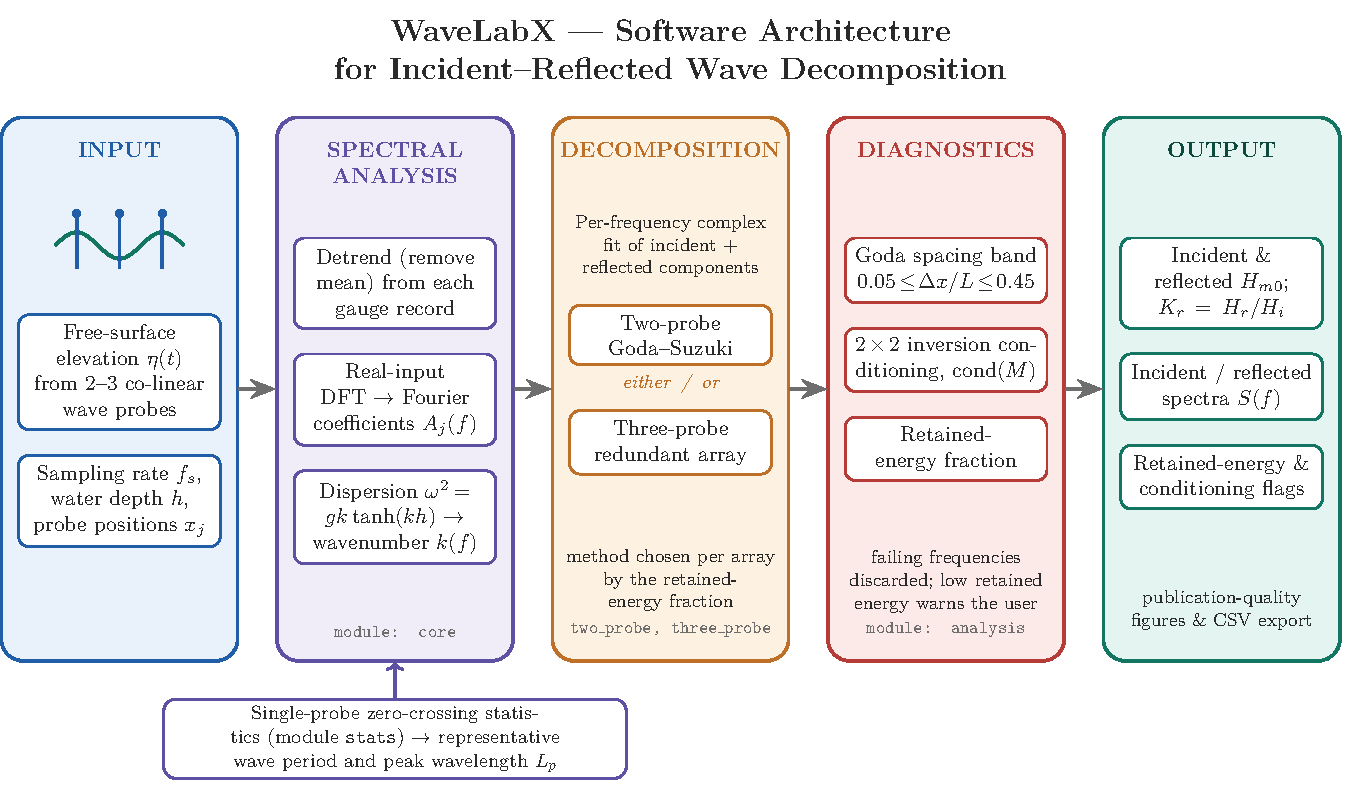
\includegraphics[width=\linewidth]{wavelabx_architecture.pdf}
\caption{WaveLabX software architecture. The analysis pipeline runs
from left to right; the two-probe and three-probe methods are a
choice, not a sequence, selected per array from the probe geometry and
the fraction of spectral energy the three-probe method retains. Both
the Python package and the browser application implement this
identical pipeline.}
\label{fig:workflow}
\end{figure}

\begin{figure}[!htbp]
\centering
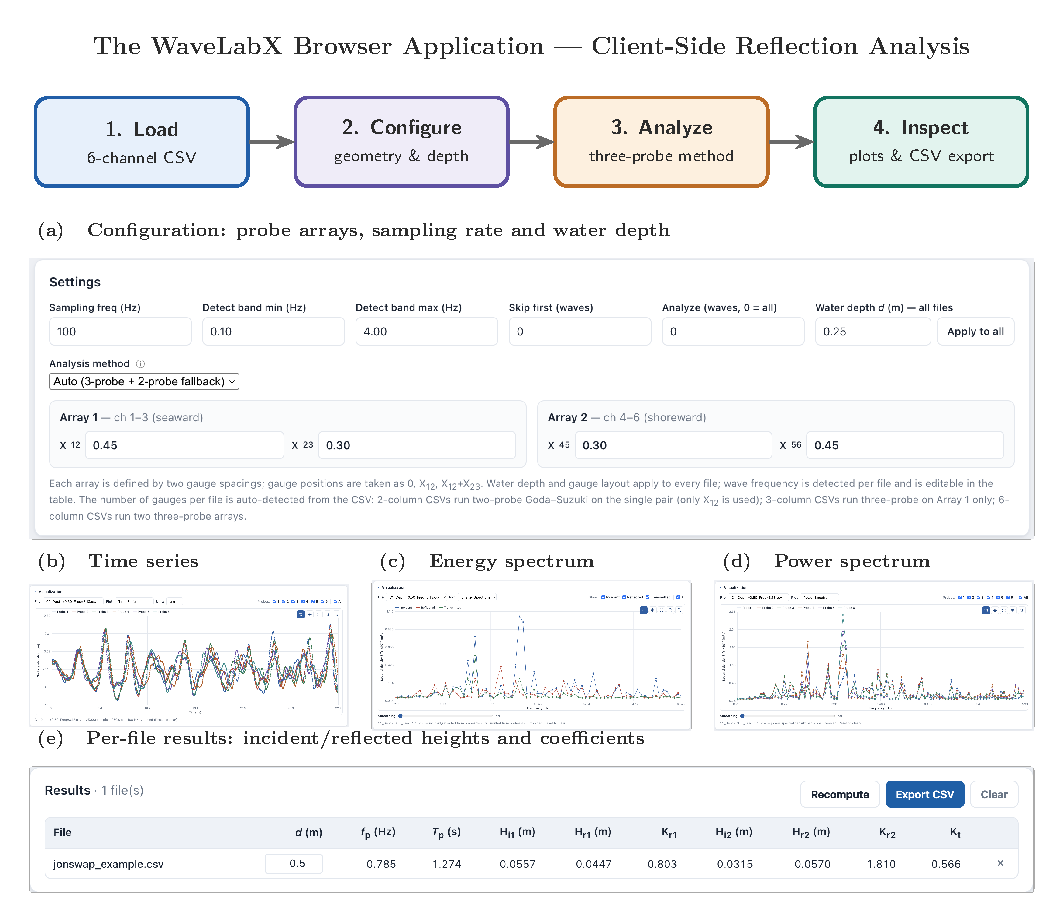
\includegraphics[width=\linewidth]{webapp_figure.pdf}
\caption{The WaveLabX browser application, applied to a six-gauge
laboratory record. The tool follows a four-step workflow: load,
configure, analyse, inspect. (a) The configuration panel sets the two
probe arrays, the sampling rate and the water depth. (b--d) The
interactive visualisation offers time-series, decomposed
incident/reflected and raw per-probe spectrum views, each with zoom,
pan and per-point readout. (e) The results table reports the incident
and reflected wave heights and the reflection coefficients of both
arrays for every file, and exports them as CSV. The application runs
entirely in the browser, with no installation and no server.}
\label{fig:webapp}
\end{figure}

% ===========================================================================
\section{Validation}
\label{sec:validation}
% ===========================================================================

\subsection{Recovery of a known synthetic truth}
Because incident and reflected components cannot be measured
independently in a physical flume, WaveLabX is validated against
synthetic three-gauge records generated from linear wave theory with
prescribed incident height, reflection coefficient and probe geometry
(\texttt{wavelabx.sensitivity}). For a well-spaced array, both methods
recover the incident and reflected spectral wave heights and the
reflection coefficient to within a few per cent of the prescribed
truth (Fig.~\ref{fig:validation}). The decomposition is therefore
shown to be correct in a controlled setting before it is applied to
laboratory data.

\begin{figure}[!htbp]
\centering
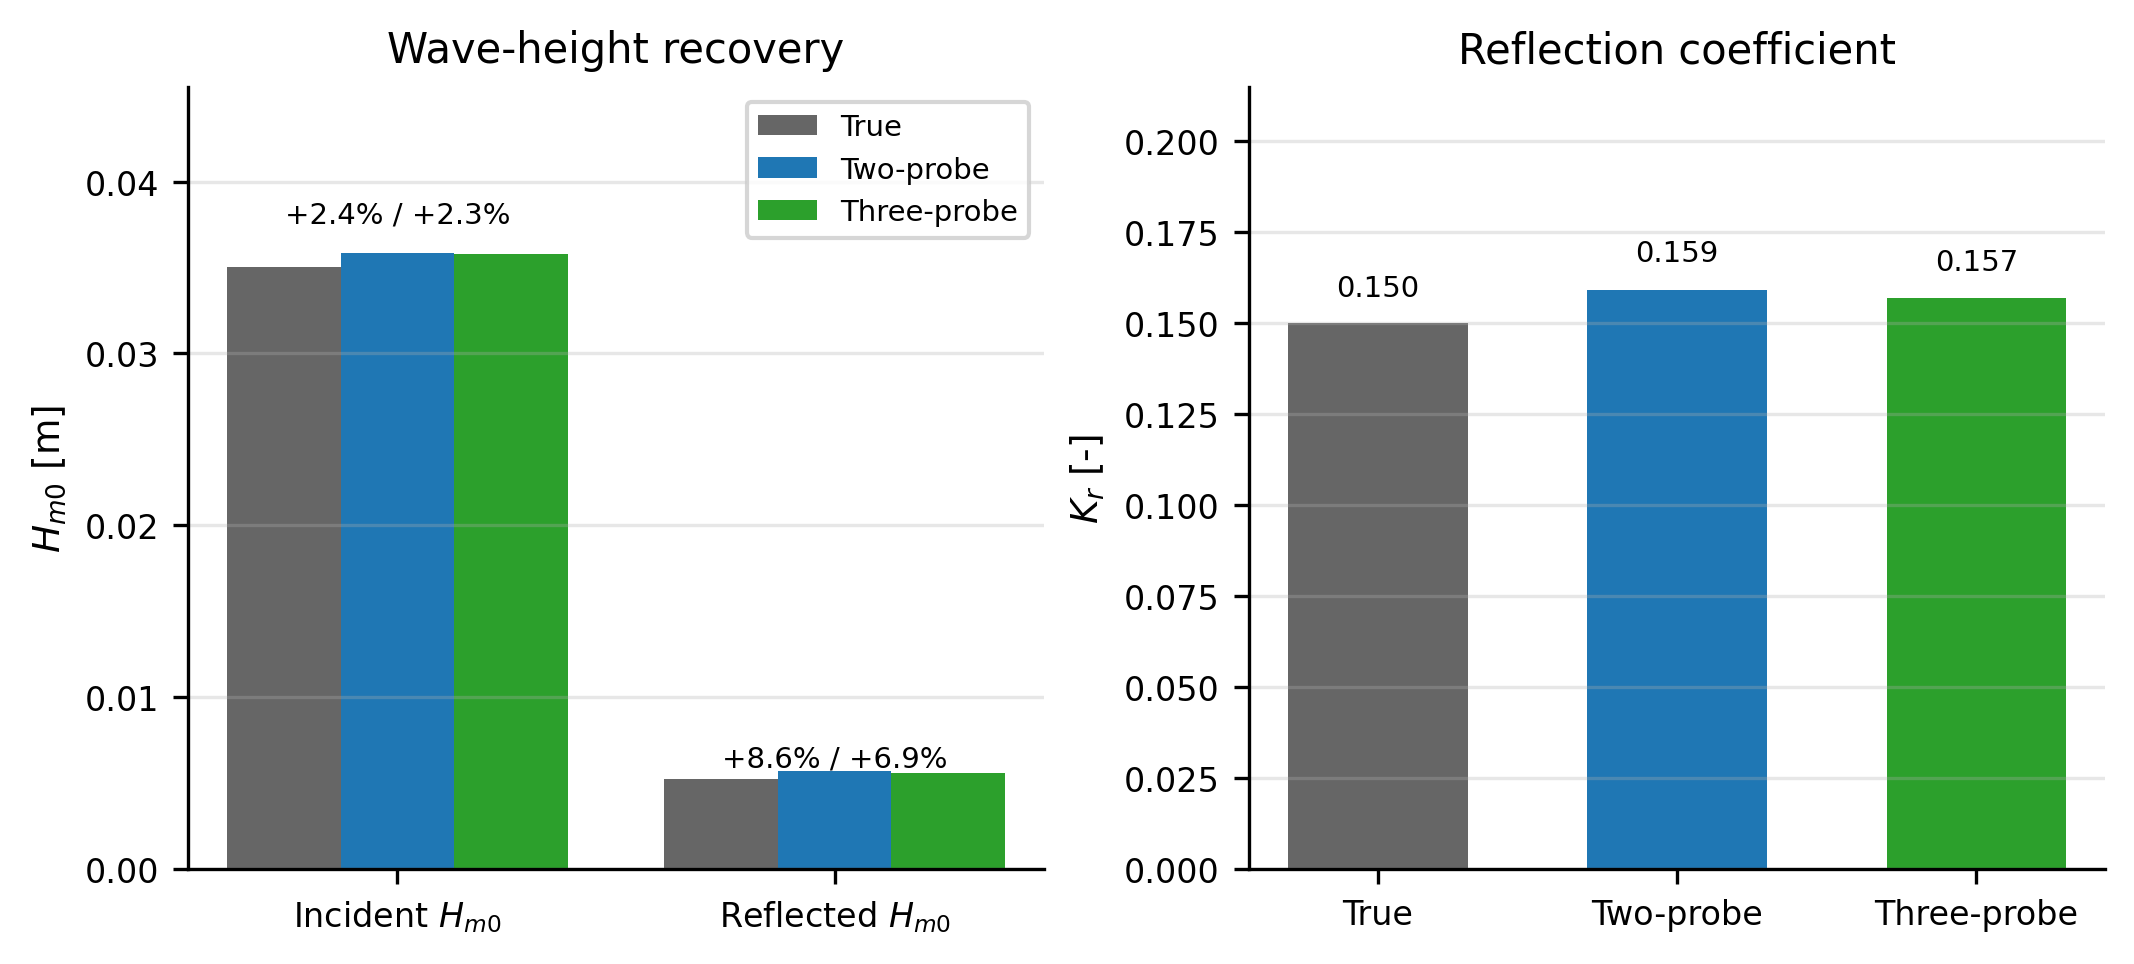
\includegraphics[width=\linewidth]{validation_known_truth.png}
\caption{Recovery of incident/reflected wave heights and the
reflection coefficient against a known synthetic truth, for a
well-spaced array. Both methods agree with the prescribed values to
within a few per cent.}
\label{fig:validation}
\end{figure}

\subsection{Probe-spacing sensitivity}
To quantify how probe spacing controls accuracy, both methods were
applied to known-truth synthetic records under deliberately different
geometric conditions (Fig.~\ref{fig:spacing}); the two panels are
designed to highlight the distinct purpose of each method.

Panel~(a) is a single-pair two-probe scan: at every $\Delta x/L$ the
gauges sit at $(0,\,\Delta x,\,2\Delta x)$ and only the first pair is
used. The recovery stays within $\pm 5\%$ for approximately
$0.07 \le \Delta x/L \le 0.36$, with one borderline point at
$\Delta x/L \approx 0.14$ reaching $\approx 5\%$; outside this range
the error degrades smoothly because the inversion approaches a
singularity.

Panel~(b) tests the redundancy of the three-probe routine on an
\emph{asymmetric} geometry: the first spacing is held fixed at
$X_{12}=0.10\,L$ (well inside the Goda band) while the second spacing
$X_{23}$ is varied across the same range as panel~(a). The routine
stays within $\pm 5\%$ across virtually the entire varied range, even
where $X_{23}$ is far outside the Goda band, because the per-frequency
masking keeps the in-band pairs and discards the out-of-band one. No
single-pair two-probe analysis can match this behaviour; this is the
redundancy benefit the three-probe method was designed for.

Both scans were repeated at three noise levels (3\%, 10\% and 30\% of
the incident height), covering typical flume signal-to-noise ratios
and a deliberately extreme stress test. Inside the recommended spacing
band the noisy two-probe curves are visually indistinguishable from
the noise-free curve up to 10\% noise; at 30\% noise a small but
visible spread appears. The three-probe panel shows almost no noise
sensitivity at any level, because the in-band pair carries the
estimate. The default retained-energy threshold of~0.8 separates the
in-band, $\pm 5\%$ regime from the regime in which the routine flags
the case automatically: at $\Delta x/L \approx 0.04$ in the
equal-spacing two-probe case, for example, the retained energy falls
below~0.4 and the result is flagged as unreliable.

\begin{figure}[!htbp]
\centering
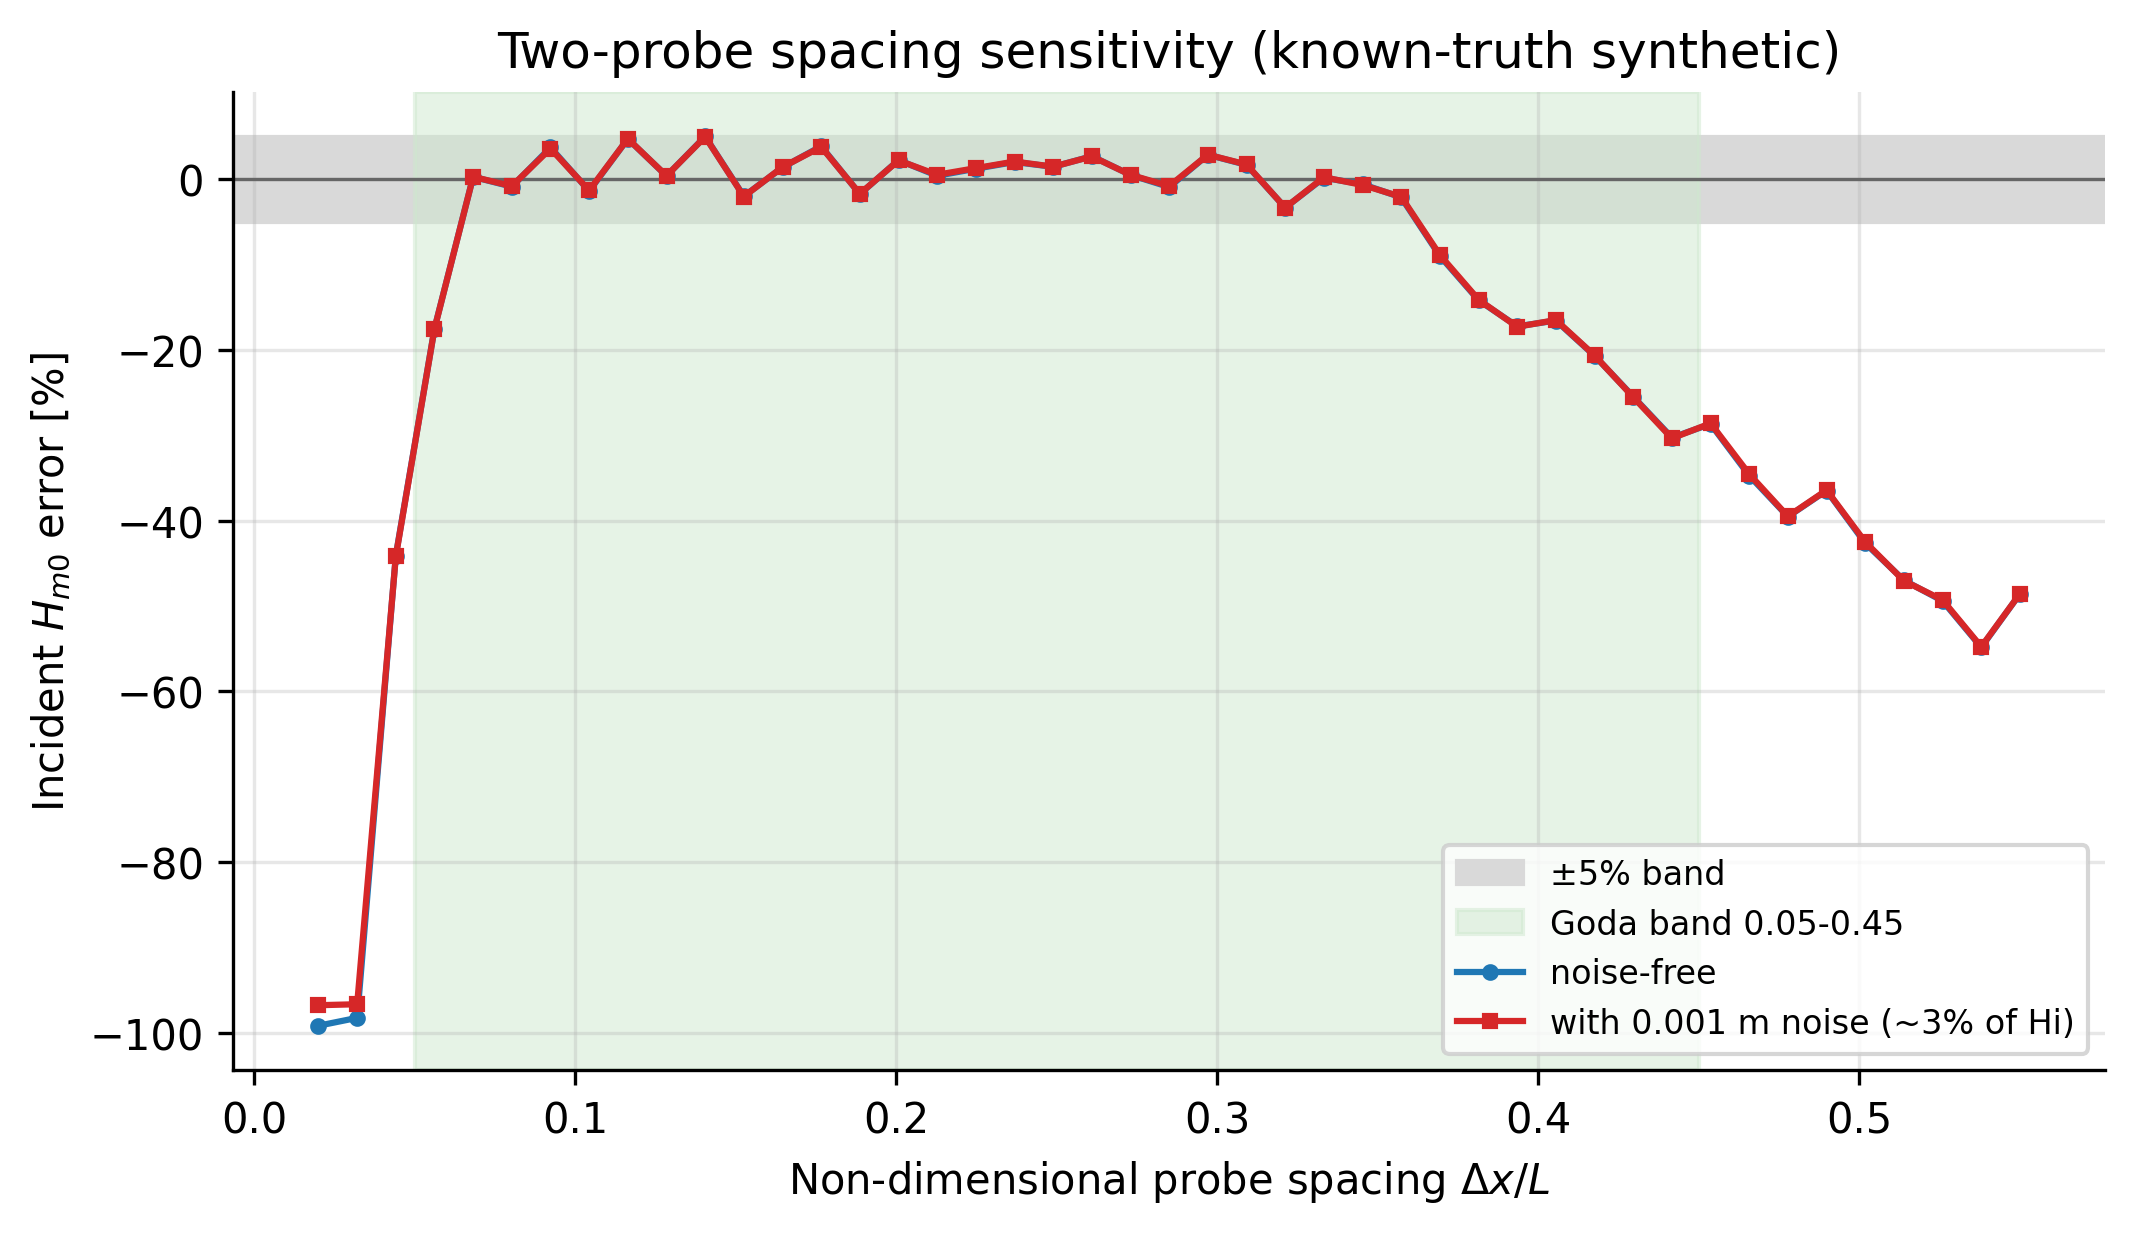
\includegraphics[width=\linewidth]{spacing_sensitivity.png}
\caption{Probe-spacing sensitivity. Panel~(a): two-probe scan with
$X_{12}=\Delta x$. Panel~(b): three-probe scan with the first spacing
held fixed at $X_{12}=0.10\,L$ (inside the Goda band) and the second
spacing $X_{23}=\Delta x$ varied across the same range. Each panel is
shown at four gauge-noise levels (noise-free, and 3\%, 10\% and 30\%
of the true incident wave height). The shaded grey band marks
$\pm 5\%$ incident-height error; the green band marks the classical
Goda spacing range $0.05 \le \Delta x/L \le 0.45$. The three-probe
panel stays inside the $\pm 5\%$ band over the entire varied range,
showing that the routine's per-frequency pair masking lets it recover
the truth even when one pair is well out of the Goda band.}
\label{fig:spacing}
\end{figure}

\subsection{Robustness on non-uniform geometries}
Beyond the varied asymmetric geometry of Fig.~\ref{fig:spacing}(b),
three representative non-uniform geometries illustrate the redundancy
benefit and the failure mode of the three-probe routine. A
well-spaced array $(0,\,0.35,\,0.70)$ keeps all three pairs inside the
band and recovers the incident height to within 3.3\%. An array of
mixed spacing $(0,\,0.10,\,0.60)$ keeps all pairs admissible and
recovers the truth to within 3.1\%. An array in which all probes are
too closely spaced $(0,\,0.05,\,0.10)$ leaves only one pair marginally
admissible: the retained-energy fraction collapses to~0.58 and the
incident height is in error by roughly 22\%, which the routine flags
through the retained-energy diagnostic. The default threshold of~0.8
is therefore not arbitrary; it is the value below which the
$\Delta x/L \in [0.07, 0.36]$ guarantee of Fig.~\ref{fig:spacing}
breaks down because no admissible pair remains.

% ===========================================================================
\section{Application to laboratory datasets}
\label{sec:application}
% ===========================================================================
\begin{sloppypar}
To exercise WaveLabX across regular, irregular and known-truth
scenarios, the three-probe method was applied to three contrasting
cases (Table~\ref{tab:cases}), all reproduced by the script
\texttt{multi\_example\_test.py} in the \texttt{scripts/} directory:
\end{sloppypar}
\begin{enumerate}[nosep,leftmargin=1.4em]
\item \emph{Synthetic regular wave with prescribed reflection.} A
monochromatic incident--reflected superposition is generated from
linear theory ($T_p=1.25$~s, $h=0.50$~m, $H_i=0.113$~m, prescribed
$K_r=0.300$) and the three-probe routine is asked to recover the
truth.
\item \emph{Real regular wave ($f=1.25$~Hz, $H_3$ target,
$h=0.35$~m).} Recorded as six-channel data at 100~Hz in
\texttt{regular\_example.csv} under \texttt{data/}; the seaward
three-gauge array (channels 1--3) is analysed with the spacings of
Fig.~\ref{fig:expsetup}, $X_{12}=0.60$~m and $X_{23}=0.30$~m.
\item \emph{Real irregular wave (JONSWAP, $h=0.50$~m).} Recorded as
six-channel data at 100~Hz in \texttt{jonswap\_example.csv} under
\texttt{data/}; the seaward array is analysed with the
browser-application default spacings $X_{12}=0.45$~m and
$X_{23}=0.30$~m.
\end{enumerate}

Fig.~\ref{fig:expsetup} shows the wave-flume layout used to acquire
the two laboratory records: a 15~m flume with a piston wavemaker at
the seaward end and an absorbing beach at the shoreward end, an
instrumented submerged structure near mid-flume, and two co-linear
three-gauge arrays (channels P1--P3 seaward and P4--P6 shoreward)
placed between the wavemaker, the structure and the beach.

\begin{sidewaysfigure}[!htbp]
\centering
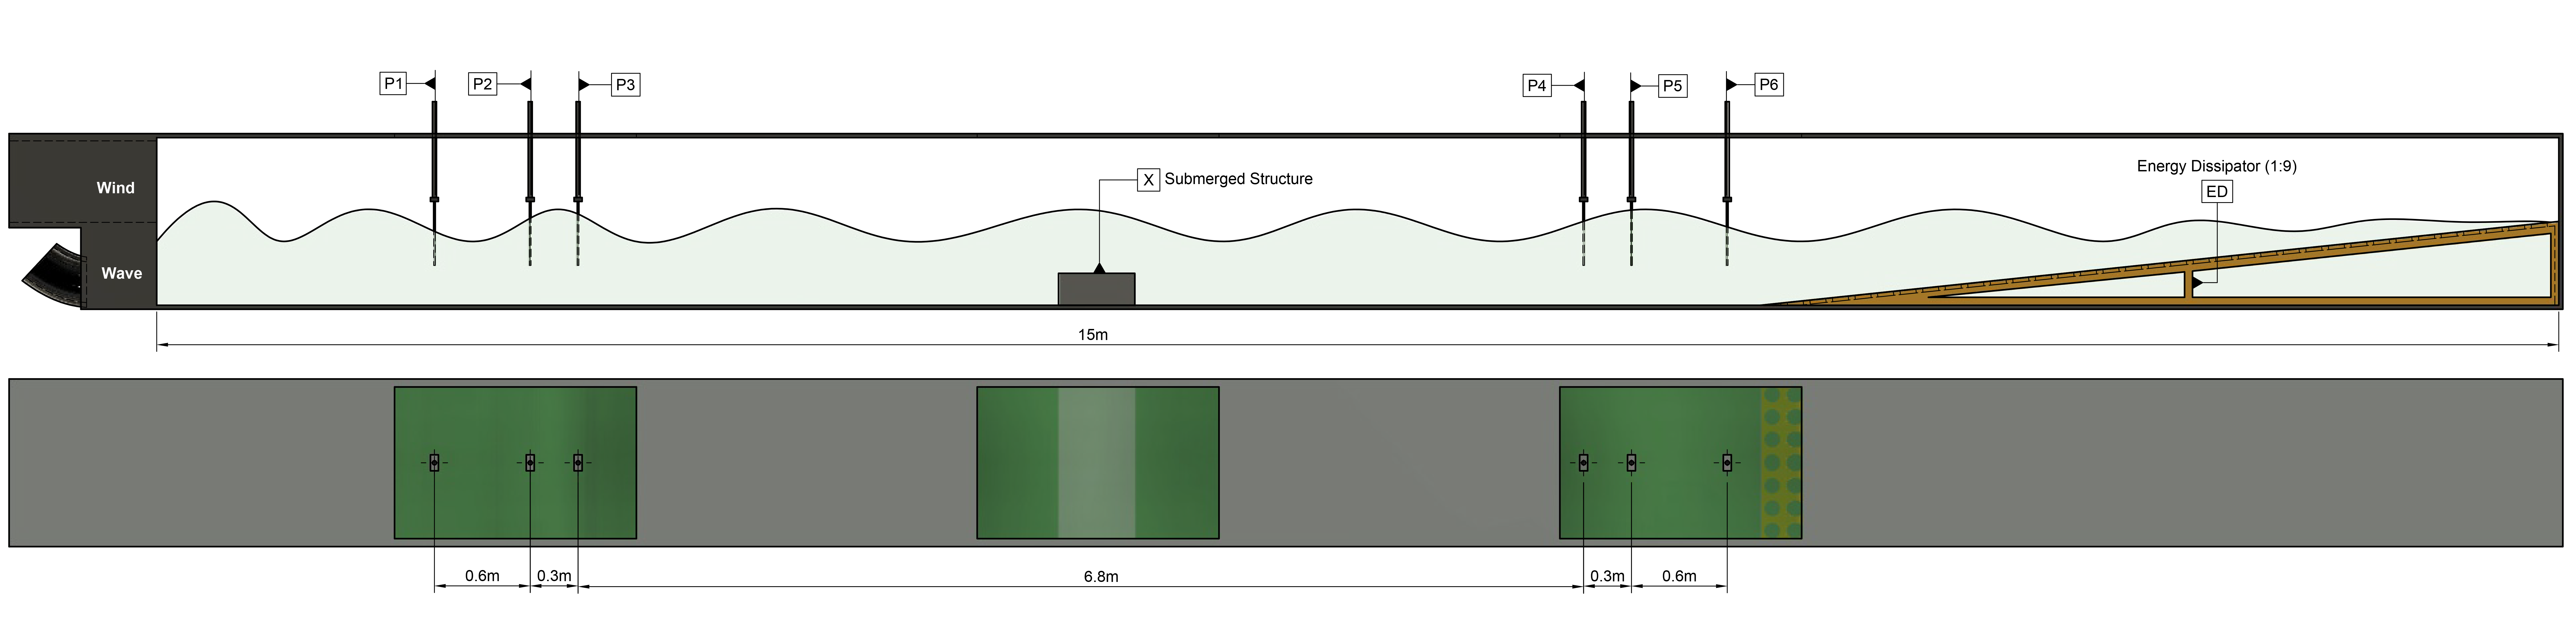
\includegraphics[width=0.95\textheight]{ExperimentalSetup.png}
\caption{Wave-flume experimental setup that produced the laboratory
records analysed in Section~\ref{sec:application}. The campaign is
described in \citet{lamsal2026seahive}. Top: elevation view, showing
the wavemaker (left), the two co-linear three-gauge probe arrays
P1--P3 and P4--P6, an instrumented submerged structure near
mid-flume, and the absorbing beach at the shoreward end. Bottom: plan
view, showing the in-flume location of each three-gauge array and the
submerged structure with measured spacings.}
\label{fig:expsetup}
\end{sidewaysfigure}

Table~\ref{tab:cases} summarises the results. The synthetic case
recovers the prescribed $K_r = 0.300$ to three decimal places, the
real regular wave is recovered with a clean physical $K_r = 0.13$ and
retained-energy fraction~0.94, and the JONSWAP array returns a
physically admissible $K_r = 0.80$ with retained-energy
fraction~0.95. Fig.~\ref{fig:spectra} shows the JONSWAP incident,
reflected and composite spectra.

\begin{table}[!htbp]
\centering
\footnotesize
\setlength{\tabcolsep}{4pt}
\resizebox{\textwidth}{!}{%
\begin{tabular}{@{}l l l l
                S[table-format=1.4] S[table-format=1.4]
                S[table-format=1.3] S[table-format=1.2]@{}}
\toprule
Case & Type & Data file & Spacings (m) &
{$H_i$ (m)} & {$H_r$ (m)} & {$K_r$} & {Retained} \\
\midrule
Synthetic regular & regular &
  \texttt{wavelabx.sensitivity} & $0.60,\,0.30$ &
  0.1131 & 0.0339 & 0.300 & 1.00 \\
Regular wave (real) & regular &
  \texttt{regular\_example.csv} & $0.60,\,0.30$ &
  0.1199 & 0.0151 & 0.126 & 0.94 \\
JONSWAP (real) & irregular &
  \texttt{jonswap\_example.csv} & $0.45,\,0.30$ &
  0.0557 & 0.0447 & 0.803 & 0.95 \\
\bottomrule
\end{tabular}}
\caption{Summary of the three illustrative cases analysed in
Section~\ref{sec:application}, the data file used and the
seaward-array gauge spacings $X_{12},X_{23}$ of each. For the
synthetic case a prescribed reflection coefficient $K_r=0.300$ was
imposed and recovered exactly. The regular-wave case uses the spacings
shown in Fig.~\ref{fig:expsetup}; the JONSWAP case uses the WaveLabX
browser-application default spacings. Data files are located under
\texttt{data/} in the repository; numbers are reproduced by
\texttt{scripts/multi\_example\_test.py} and stored in
\texttt{results/multi\_example\_results.csv}.}
\label{tab:cases}
\end{table}

The regular-wave case illustrates the diagnostic in action. At
$f=1.25$~Hz and $h=0.35$~m the wavelength is $L\approx 0.98$~m, so the
three pairs sit at $\Delta x/L\approx 0.61$, $0.92$ and $0.31$; only
pair~(2--3) lies inside the Goda band
$0.05\le\Delta x/L\le 0.45$. Per-frequency masking inside
\texttt{three\_probe\_array} reduces the calculation at the dominant
frequency to a single-pair estimate on pair~(2--3), and the
retained-energy fraction of~0.94 confirms that nearly all spectral
energy is admissible. That the synthetic case recovers $K_r=0.300$
exactly under the same conditions shows the single-pair fallback to be
self-consistent. The per-pair Goda warning emitted by both the Python
package and the browser application makes this state visible at a
glance.

\begin{figure}[!htbp]
\centering
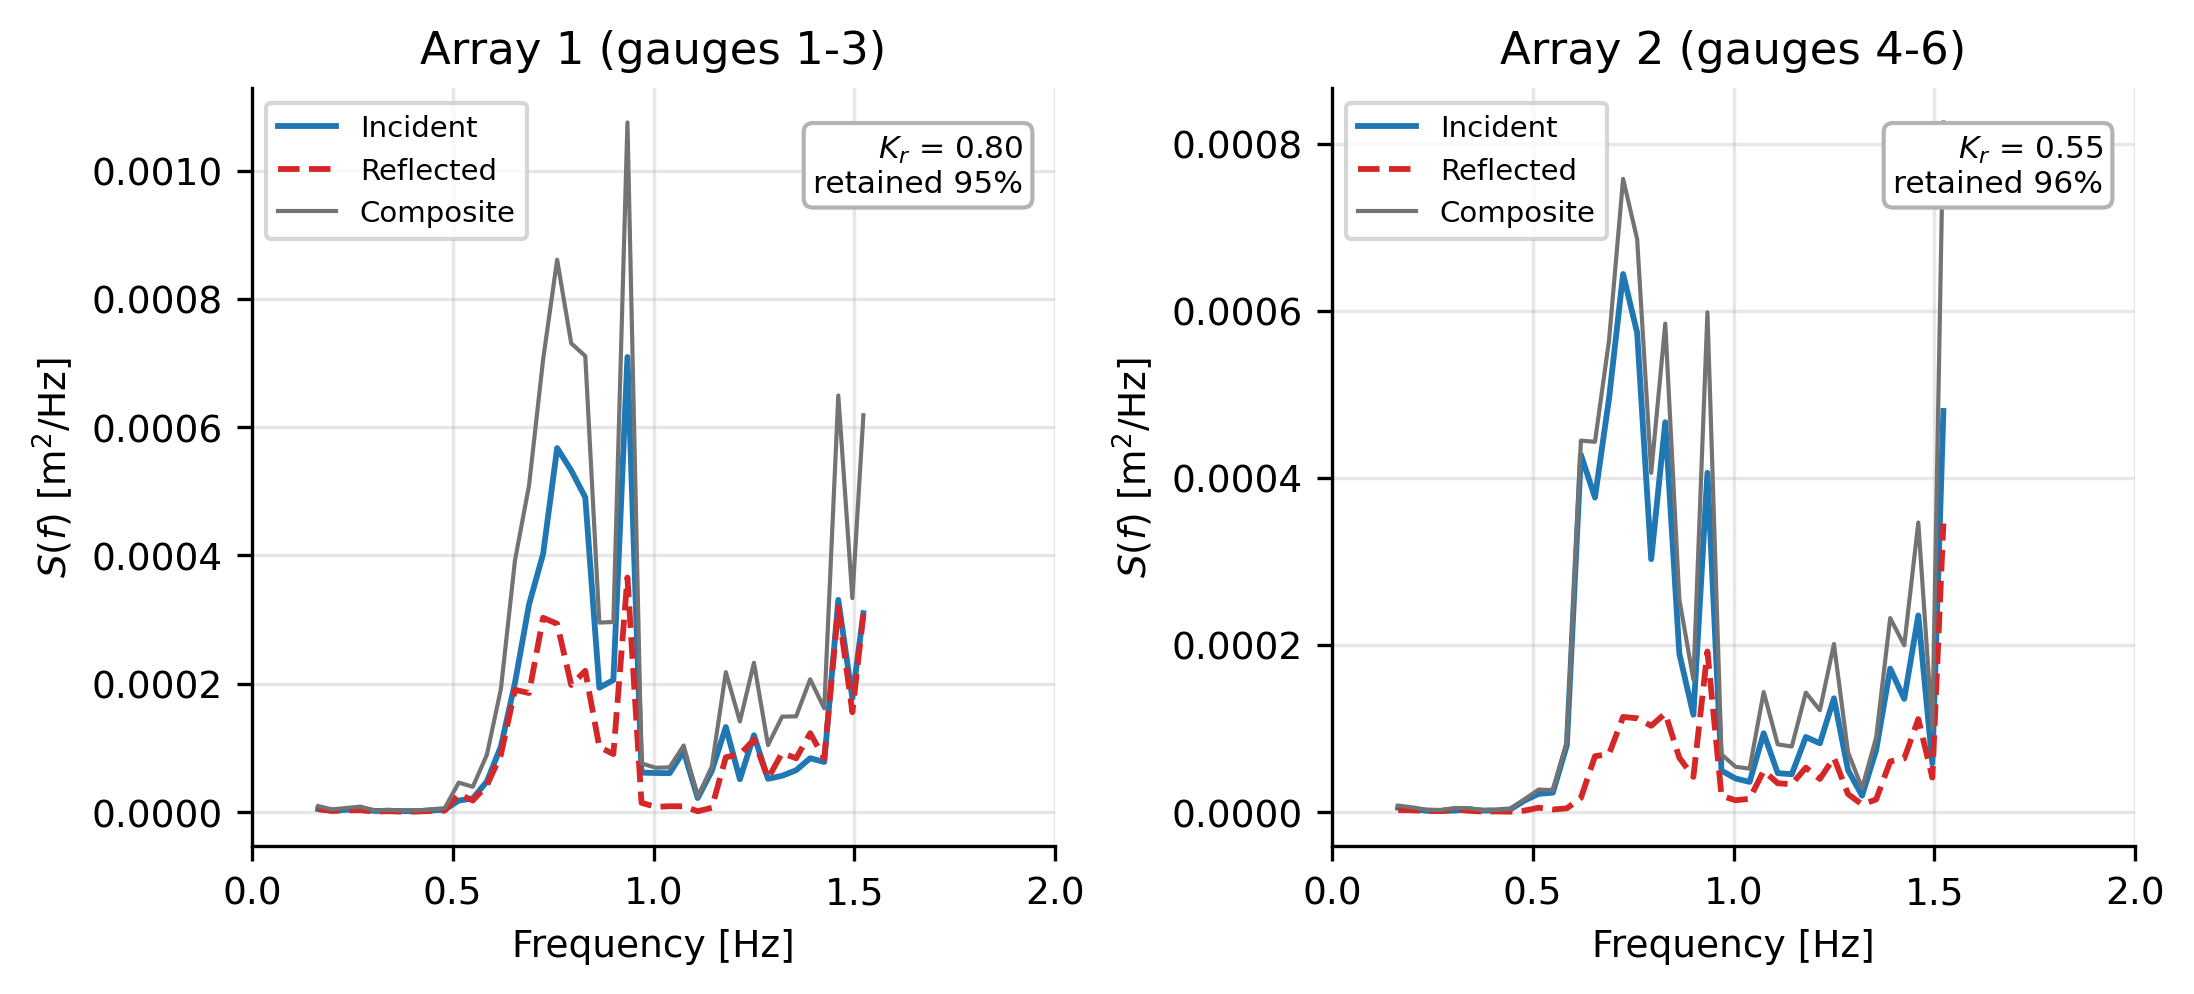
\includegraphics[width=0.75\linewidth]{realdata_spectra.png}
\caption{Incident, reflected and composite wave spectra from the real
irregular-wave (JONSWAP) laboratory record
\texttt{data/jonswap\_example.csv}, computed for the seaward
three-gauge array (channels 1--3).}
\label{fig:spectra}
\end{figure}

% ===========================================================================
\section{Discussion}
\label{sec:discussion}
% ===========================================================================
The validation and application results lead to three observations of
practical relevance for laboratory wave analysis.

\paragraph{The Goda band is a necessary but not sufficient condition.}
Within the textbook band $0.05 \le \Delta x/L \le 0.45$ the two-probe
inversion can still be ill-conditioned at specific frequencies, and a
single-pair analysis can drift outside $\pm 5\%$ near the band edges
even in the absence of noise (Fig.~\ref{fig:spacing}a). A practical
implementation that returns only the inverted coefficients, without an
explicit conditioning test, therefore embeds an unflagged source of
error. The condition-number filter applied at every frequency in
WaveLabX, together with the retained-energy fraction reported with the
estimate, makes this source of error observable.

\paragraph{The three-probe method earns its complexity through its
diagnostics.} If all three pairs of a three-probe array satisfy the
Goda band, the three-probe method is a modest accuracy improvement
over the best two-probe pair. Its decisive advantage emerges when the
array is non-uniform, as is common in practice, where the per-pair
masking inside \texttt{three\_probe\_array} keeps the in-band pairs
and discards the out-of-band ones automatically
(Fig.~\ref{fig:spacing}b). The cost is the bookkeeping of three
$2\times 2$ inversions per frequency; the benefit is a result with a
self-reported retained-energy fraction, that is, a quantitative
estimate of the spectral fraction on which the decomposition was
actually performed.

\paragraph{The retained-energy threshold is a design-time tool.} The
spacing-sensitivity and non-uniform-geometry results indicate that the
default threshold of~0.8 is the value below which the
$\Delta x/L \in [0.07, 0.36]$ guarantee of Fig.~\ref{fig:spacing}
breaks down because no admissible pair remains. Experimentalists can
use this criterion not only after the test, to flag an unreliable
estimate, but also before the test, when choosing probe positions:
running the spacing scan in \texttt{wavelabx.sensitivity} for the
target period range identifies geometries that will return
retained-energy fractions above~0.8 across the spectrum, and is a
practical alternative to repeatedly re-running an entire campaign with
suboptimally placed probes.

The software was developed alongside laboratory programs at the
SUSTAIN Laboratory of the University of Miami and has supported a body
of experimental wave--structure-interaction research, including studies
of submerged SEAHIVE breakwaters \citep{lamsal2026seahive}, perforated
breakwater structures \citep{lamsal2024quantifying}, hybrid coral-reef
structures \citep{lamsal2024hybridcoral}, wave dissipation by mangrove
forests \citep{clark2024wave}, hurricane-induced wind and wave loading
\citep{aguilar2024hurricane}, beach-erosion-control modelling and
design \citep{ghiasian2026beach}, and a doctoral dissertation on
submerged breakwaters for coastal protection
\citep{lamsal2025dissertation}; the toolkit itself is openly archived
\citep{lamsal2025wavelabx}.

WaveLabX targets one-dimensional wave propagation with co-linear probe
arrays and linear-wave behaviour; strongly nonlinear waves, breaking
and multi-directional wave fields are outside its current scope. The
embedded diagnostics also rely on the linear superposition assumed by
the Goda--Suzuki and three-probe formulations; their reliability under
strongly nonlinear conditions is a topic for future work.

% ===========================================================================
\section{Conclusions}
\label{sec:conclusions}
% ===========================================================================
This work presented WaveLabX, an open-source toolkit that unifies
zero-crossing wave statistics with two- and three-probe
incident--reflected decomposition under one spectral formulation.
Reliability diagnostics---probe-spacing checks, inversion conditioning
and a retained-energy fraction---are embedded directly in the
analysis, attaching a quantitative measure of trust to every estimate.

Validation against synthetic records with prescribed reflection
coefficients showed that both methods recover incident and reflected
wave heights to within a few per cent for well-conditioned arrays;
that the two-probe error grows predictably outside the spacing range
$0.07 \le \Delta x/L \le 0.36$; and that the three-probe method's
per-frequency masking keeps the estimate within $\pm 5\%$ even when
one pair is far outside the Goda band, because the masking discards
that pair automatically. Application to laboratory records of one
regular wave and one JONSWAP-shaped irregular wave produced
physically admissible reflection coefficients with retained-energy
fractions above~0.9, and demonstrated that the per-pair Goda
diagnostic correctly identified the configurations in which the
estimate reduced to a single admissible pair.

Distributed as a Python package and a zero-install browser
application---the two interfaces sharing an automated numerical
cross-check---WaveLabX is intended to support reproducible reflection
analysis across coastal- and hydraulic-engineering laboratories.
Future work includes extending the methods to oblique and
multi-directional wave fields.

\section*{Data and code availability}
\begin{sloppypar}
The WaveLabX source code, example datasets, reproducible scripts and
the browser application are openly available under the MIT License at
\url{https://github.com/sandslamsal/WaveLabX}. The version that
supports the figures, tables and analyses reported in this manuscript
is archived on Zenodo as \citet{lamsal2025wavelabx}
(\href{https://doi.org/10.5281/zenodo.20217994}{doi:10.5281/zenodo.20217994}).
The example records analysed in Section~\ref{sec:application}
(\texttt{regular\_example.csv} and \texttt{jonswap\_example.csv} under
the \texttt{data/} directory) are bundled with the release. Running
\texttt{multi\_example\_test.py} under \texttt{scripts/} regenerates
the numerical results in Table~\ref{tab:cases}; running
\texttt{real\_data\_example.py} regenerates the spectra in
Fig.~\ref{fig:spectra}. The browser application is deployed at
\url{https://wave-lab-x.vercel.app} and runs the same analysis routine
as the Python package.
\end{sloppypar}

\section*{Acknowledgements}
The development of WaveLabX was motivated by experimental workflows
used in the SUSTAIN Laboratory at the University of Miami. The authors
thank colleagues and technical staff who supported the laboratory
programs that informed the design of this software.

% ---------------------------------------------------------------------------
\FloatBarrier
\bibliographystyle{elsarticle-harv}
\bibliography{paper}

\end{document}
